% So I have up to 11 texts I need to show here
% lut64
% pext64
% shuffle64
% shuffle128
% shuffle256
% shuffle512
% pc
% pc-ss
% ps
% kaneta-pext
% kaneta-pshufb

\documentclass[a4]{article}

\usepackage[utf8]{inputenc}
\usepackage[english]{babel}

\usepackage{amsmath,amsfonts,amssymb}
\usepackage{fullpage}
\usepackage{verbatim}

\usepackage{tikz,pgfplots}
\usetikzlibrary{patterns, patterns.meta}
\usepgfplotslibrary{groupplots}



\pgfplotsset{
    width = 150mm,
    height = 100mm,
    major grid style = { thin, dotted, color = black!50 },
    minor grid style = { thin, dotted, color = black!50 },
    grid,
    xtick distance = 1,
    ytick distance = 200,
    ymin = 0,
    legend cell align = left,
    legend pos = north west,
	  /pgfplots/ybar legend/.style = {
		  /pgfplots/legend image code/.code={%
			  \draw[##1,/tikz/.cd,yshift=-0.35em]
      (0cm,0cm) rectangle (0.7em,0.8em);},
	  },  
}


\begin{document}

\title{WT Benchmark}
\author{Jan-Philipp Tarnowski}
\maketitle

\clearpage


% IMPORT-DATA stats ../results-pcc-regular.out
% IMPORT-DATA stats_large ../results-large.out
% IMPORT-DATA stats_lw ../results-lightweight-regular.out
% IMPORT-DATA stats_ru ../results-ru-regular.out

% SQL INSERT INTO stats SELECT * FROM stats_large
% SQL INSERT INTO stats SELECT * FROM stats_lw
% SQL INSERT INTO stats SELECT * FROM stats_ru

% SQL UPDATE stats SET file = 'dblp.xml' WHERE file LIKE '%/dblp.xml'
% SQL UPDATE stats SET file = 'dna' WHERE file LIKE '%/dna'
% SQL UPDATE stats SET file = 'english' WHERE file LIKE '%/english'
% SQL UPDATE stats SET file = 'pitches' WHERE file LIKE '%/pitches'
% SQL UPDATE stats SET file = 'proteins' WHERE file LIKE '%/proteins'
% SQL UPDATE stats SET file = 'sources' WHERE file LIKE '%/sources'

% SQL UPDATE stats SET file = 'chr22.dna' WHERE file LIKE '%/chr22.dna'
% SQL UPDATE stats SET file = 'etext99' WHERE file LIKE '%/etext99'
% SQL UPDATE stats SET file = 'gcc-3.0.tar' WHERE file LIKE '%/gcc-3.0.tar'
% SQL UPDATE stats SET file = 'howto' WHERE file LIKE '%/howto'
% SQL UPDATE stats SET file = 'jdk13c' WHERE file LIKE '%/jdk13c'
% SQL UPDATE stats SET file = 'linux-2.4.5.tar' WHERE file LIKE '%/linux-2.4.5.tar'
% SQL UPDATE stats SET file = 'rctail96' WHERE file LIKE '%/rctail96'
% SQL UPDATE stats SET file = 'rfc' WHERE file LIKE '%/rfc'
% SQL UPDATE stats SET file = 'sprot34.dat' WHERE file LIKE '%/sprot34.dat'
% SQL UPDATE stats SET file = 'w3c2' WHERE file LIKE '%/w3c2'

% SQL UPDATE stats SET file = 'cc.16gib' WHERE file LIKE '%/cc.txt'
% SQL UPDATE stats SET file = 'dna.16gib' WHERE file LIKE '%/dna.txt'
% SQL UPDATE stats SET file = 'wiki.16gib' WHERE file LIKE '%/wiki.txt'
% SQL UPDATE stats SET file = 'ru.8gib' WHERE file LIKE '%/ru.wo_punct.wb'

% SQL UPDATE stats SET type = 'lwt-lut-16-4-4', ds_order = 0 WHERE type LIKE 'lwt_lut_16_4_4'
% SQL UPDATE stats SET type = 'lwt-pext-16-4', ds_order = 1 WHERE type LIKE 'lwt_pext_16_4'
% SQL UPDATE stats SET type = 'lwt-shuffle-8-8', ds_order = 2 WHERE type LIKE 'lwt_shuffle_8_8'
% SQL UPDATE stats SET type = 'lwt-shuffle-16-8', ds_order = 3 WHERE type LIKE 'lwt_shuffle_16_8'
% SQL UPDATE stats SET type = 'lwt-shuffle-32-8', ds_order = 4 WHERE type LIKE 'lwt_shuffle_32_8'
% SQL UPDATE stats SET type = 'lwt-shuffle-64-8', ds_order = 5 WHERE type LIKE 'lwt_shuffle_64_8'

% SQL UPDATE stats SET type = 'pwm-pc-tree', ds_order = 6 WHERE type LIKE 'pwm__wx_pc________tree'
% SQL UPDATE stats SET type = 'pwm-pc-ss-tree', ds_order = 7 WHERE type LIKE 'pwm__wx_pc_ss________tree'
% SQL UPDATE stats SET type = 'pwm-ps-tree', ds_order = 8 WHERE type LIKE 'pwm__wx_ps________tree'


% SQL UPDATE stats SET type = 'wm-lut-16-4-4', ds_order = 9 WHERE type LIKE 'wm_lut_16_4_4'
% SQL UPDATE stats SET type = 'wm-pext-8-8', ds_order = 10 WHERE type LIKE 'wm_pext_8_8'
% SQL UPDATE stats SET type = 'wm-shuffle-8-8', ds_order = 11 WHERE type LIKE 'wm_shuffle_8_8'
% SQL UPDATE stats SET type = 'wm-shuffle-16-8', ds_order = 12 WHERE type LIKE 'wm_shuffle_16_8'
% SQL UPDATE stats SET type = 'wm-shuffle-32-8', ds_order = 13 WHERE type LIKE 'wm_shuffle_32_8'
% SQL UPDATE stats SET type = 'wm-shuffle-64-8', ds_order = 14 WHERE type LIKE 'wm_shuffle_64_8'

% SQL UPDATE stats SET type = 'pwm-pc-matrix', ds_order = 15 WHERE type LIKE 'pwm__wx_pc________matrix'
% SQL UPDATE stats SET type = 'pwm-pc-ss-matrix', ds_order = 16 WHERE type LIKE 'pwm__wx_pc_ss________matrix'
% SQL UPDATE stats SET type = 'pwm-ps-matrix', ds_order = 17 WHERE type LIKE 'pwm__wx_ps________matrix'

% SQL DELETE FROM stats WHERE type LIKE '%\_%' ESCAPE '\'


\pgfplotsset{
  /pgfplots/bar cycle list/.style = {
    /pgfplots/cycle list = {
      { fill = red!50, mark = none },          % LUT
      { fill = green!65, mark = none },        % PEXT
      { fill = blue!55, mark = none },         % PSHUFB 8-8
      { fill = orange!65, mark = none },       % PSHUFB 16-8
      { fill = violet!60, mark = none },       % PSHUFB 32-8
      { fill = yellow!80, mark = none },       % PSHUFB 64-8
      { fill = blue!50!green!75, mark = none },% PWM PC
      { fill = red!75!blue!50, mark = none },  % PWM PC SS
      { fill = brown!50, mark = none },        % PWM PS
      { fill = red!50, mark = none },          % KANETA PEXT
      { fill = orange!50, mark = none }        % KANETA PSHUFB
    }
  }
}

\begin{figure}
\begin{center}
    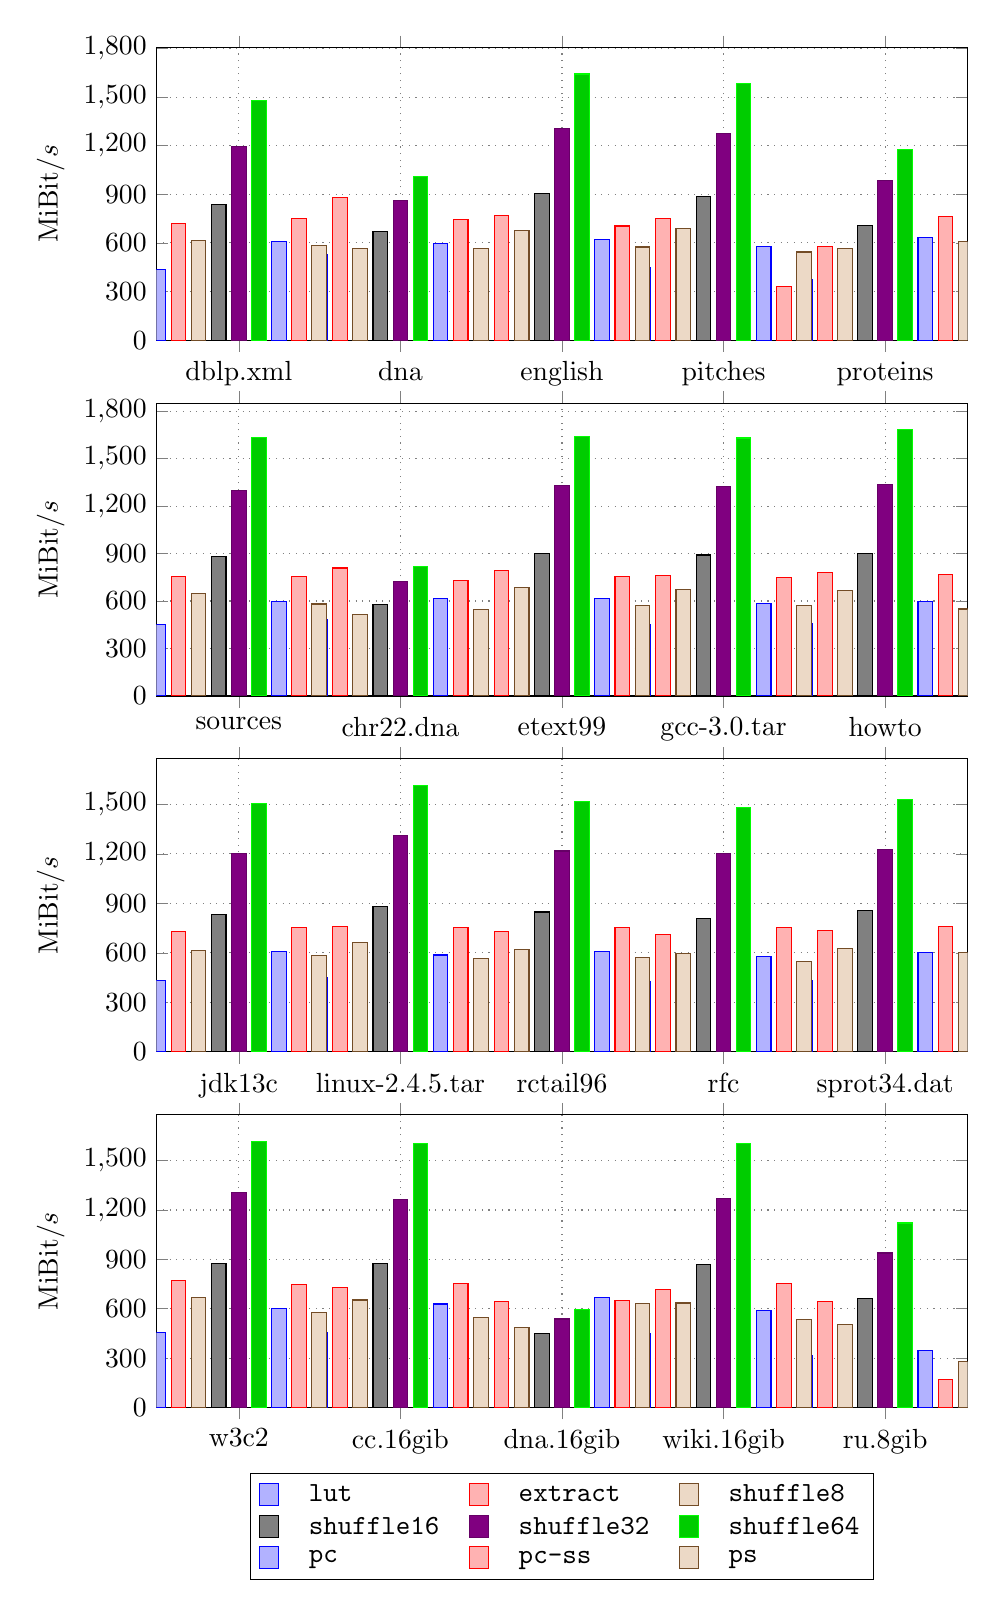
\begin{tikzpicture}
        \begin{groupplot} [
            width = 0.98\textwidth,
            height = 5.3cm,
            ybar,
            enlarge x limits = 0.1275,
            group style = { 
                vertical sep = 0.8cm,
                group size = { 
                    1 by 4
                } 
            },
            ylabel = $\text{MiBit}/s$,
            legend style = { 
                at = {(0.5, -0.225)},
                anchor = north,
                legend columns = 3,
                column sep = 2ex
            },
            ytick distance = 300,
            symbolic x coords = {
                dblp.xml,
                dna,
                english,
                pitches,
                proteins,
                sources,
                chr22.dna,
                etext99,
                gcc-3.0.tar,
                howto,
                jdk13c,
                linux-2.4.5.tar,
                rctail96,
                rfc,
                sprot34.dat,
                w3c2,
                cc.16gib,
                dna.16gib,
                wiki.16gib,
                ru.8gib
            }
        ]
        
        
        \nextgroupplot [
            bar width = 0.185cm
        ]


			%% MULTIPLOT(type) SELECT file AS x, MEDIAN((height * (size / CAST(time_in_s AS Float))) / (1024 * 1024)) AS y,MULTIPLOT
			%% FROM stats WHERE (type LIKE 'lwt%' OR type LIKE '%tree') AND (file LIKE 'dblp.xml' OR file LIKE 'dna' OR file LIKE 'english' OR file LIKE 'pitches' OR file LIKE 'proteins') GROUP BY MULTIPLOT,x ORDER BY ds_order,MULTIPLOT,x
   \addplot coordinates { (dblp.xml,433.435) (dna,529.317) (english,456.909) (pitches,448.023) (proteins,375.731) };
   \addlegendentry{type=lwt-lut-16-4-4};
   \addplot coordinates { (dblp.xml,722.205) (dna,883) (english,770.548) (pitches,749.238) (proteins,575.985) };
   \addlegendentry{type=lwt-pext-16-4};
   \addplot coordinates { (dblp.xml,614.24) (dna,563.111) (english,677.957) (pitches,686.877) (proteins,565.628) };
   \addlegendentry{type=lwt-shuffle-8-8};
   \addplot coordinates { (dblp.xml,834.915) (dna,668.928) (english,906.417) (pitches,886.621) (proteins,707.231) };
   \addlegendentry{type=lwt-shuffle-16-8};
   \addplot coordinates { (dblp.xml,1197.8) (dna,862.494) (english,1304.8) (pitches,1276.36) (proteins,985.354) };
   \addlegendentry{type=lwt-shuffle-32-8};
   \addplot coordinates { (dblp.xml,1477.77) (dna,1011.45) (english,1642.69) (pitches,1584.19) (proteins,1178.02) };
   \addlegendentry{type=lwt-shuffle-64-8};
   \addplot coordinates { (dblp.xml,608.433) (dna,594.015) (english,623.076) (pitches,578.704) (proteins,633.578) };
   \addlegendentry{type=pwm-pc-tree};
   \addplot coordinates { (dblp.xml,752.479) (dna,745.682) (english,704.904) (pitches,328.468) (proteins,761.408) };
   \addlegendentry{type=pwm-pc-ss-tree};
   \addplot coordinates { (dblp.xml,584.499) (dna,564.818) (english,574.721) (pitches,544.345) (proteins,606.68) };
   \addlegendentry{type=pwm-ps-tree};


    \legend{};

   \nextgroupplot [
    bar width = 0.185cm
]


    %% MULTIPLOT(type) SELECT file AS x, MEDIAN((height * (size / CAST(time_in_s AS Float))) / (1024 * 1024)) AS y,MULTIPLOT
    %% FROM stats WHERE (type LIKE 'lwt%' OR type LIKE '%tree') AND (file LIKE 'sources' OR file LIKE 'chr22.dna' OR file LIKE 'etext99' OR file LIKE 'gcc-3.0.tar' OR file LIKE 'howto') GROUP BY MULTIPLOT,x ORDER BY ds_order,MULTIPLOT,x
    \addplot coordinates { (chr22.dna,480.584) (etext99,461.467) (gcc-3.0.tar,453.094) (howto,457.518) (sources,451.243) };
    \addlegendentry{type=lwt-lut-16-4-4};
    \addplot coordinates { (chr22.dna,808.538) (etext99,790.826) (gcc-3.0.tar,760.615) (howto,779.279) (sources,757.753) };
    \addlegendentry{type=lwt-pext-16-4};
    \addplot coordinates { (chr22.dna,514.561) (etext99,687.514) (gcc-3.0.tar,673.4) (howto,667.552) (sources,650.216) };
    \addlegendentry{type=lwt-shuffle-8-8};
    \addplot coordinates { (chr22.dna,579.078) (etext99,899.975) (gcc-3.0.tar,890.667) (howto,902.569) (sources,882.454) };
    \addlegendentry{type=lwt-shuffle-16-8};
    \addplot coordinates { (chr22.dna,724.046) (etext99,1330.28) (gcc-3.0.tar,1325.96) (howto,1336.93) (sources,1296.8) };
    \addlegendentry{type=lwt-shuffle-32-8};
    \addplot coordinates { (chr22.dna,815.662) (etext99,1640.15) (gcc-3.0.tar,1629.95) (howto,1682.26) (sources,1632.85) };
    \addlegendentry{type=lwt-shuffle-64-8};
    \addplot coordinates { (chr22.dna,617.507) (etext99,616.842) (gcc-3.0.tar,586.916) (howto,599.334) (sources,594.222) };
    \addlegendentry{type=pwm-pc-tree};
    \addplot coordinates { (chr22.dna,731.775) (etext99,752.478) (gcc-3.0.tar,750.557) (howto,768.495) (sources,754.717) };
    \addlegendentry{type=pwm-pc-ss-tree};
    \addplot coordinates { (chr22.dna,546.645) (etext99,572.073) (gcc-3.0.tar,573.253) (howto,549.373) (sources,580.835) };
    \addlegendentry{type=pwm-ps-tree};


    \legend{};

    \nextgroupplot [
        bar width = 0.185cm
    ]

    
    
        %% MULTIPLOT(type) SELECT file AS x, MEDIAN((height * (size / CAST(time_in_s AS Float))) / (1024 * 1024)) AS y,MULTIPLOT
        %% FROM stats WHERE (type LIKE 'lwt%' OR type LIKE '%tree') AND (file LIKE 'jdk13c' OR file LIKE 'sprot34.dat' OR file LIKE 'linux-2.4.5.tar' OR file LIKE 'rctail96' OR file LIKE 'rfc') GROUP BY MULTIPLOT,x ORDER BY ds_order,MULTIPLOT,x
        \addplot coordinates { (jdk13c,433.603) (linux-2.4.5.tar,452.087) (rctail96,434.32) (rfc,424.99) (sprot34.dat,433.667) };
        \addlegendentry{type=lwt-lut-16-4-4};
        \addplot coordinates { (jdk13c,726.537) (linux-2.4.5.tar,758.871) (rctail96,728.71) (rfc,709.137) (sprot34.dat,736.44) };
        \addlegendentry{type=lwt-pext-16-4};
        \addplot coordinates { (jdk13c,613.813) (linux-2.4.5.tar,663.42) (rctail96,620.496) (rfc,596.415) (sprot34.dat,626.154) };
        \addlegendentry{type=lwt-shuffle-8-8};
        \addplot coordinates { (jdk13c,831.291) (linux-2.4.5.tar,878.371) (rctail96,847.545) (rfc,808.32) (sprot34.dat,857.029) };
        \addlegendentry{type=lwt-shuffle-16-8};
        \addplot coordinates { (jdk13c,1203.99) (linux-2.4.5.tar,1309.07) (rctail96,1217.42) (rfc,1201.2) (sprot34.dat,1224.69) };
        \addlegendentry{type=lwt-shuffle-32-8};
        \addplot coordinates { (jdk13c,1505.99) (linux-2.4.5.tar,1614.02) (rctail96,1516.18) (rfc,1478.66) (sprot34.dat,1528.5) };
        \addlegendentry{type=lwt-shuffle-64-8};
        \addplot coordinates { (jdk13c,608.552) (linux-2.4.5.tar,586.249) (rctail96,607.049) (rfc,578.153) (sprot34.dat,602.531) };
        \addlegendentry{type=pwm-pc-tree};
        \addplot coordinates { (jdk13c,752.444) (linux-2.4.5.tar,751.254) (rctail96,754.894) (rfc,752.824) (sprot34.dat,759.345) };
        \addlegendentry{type=pwm-pc-ss-tree};
        \addplot coordinates { (jdk13c,580.91) (linux-2.4.5.tar,564.751) (rctail96,571.661) (rfc,549.818) (sprot34.dat,600.563) };
        \addlegendentry{type=pwm-ps-tree};


        \legend{};


        \nextgroupplot [
            bar width = 0.185cm,
        ]
    
        
        
            %% MULTIPLOT(type) SELECT file AS x, MEDIAN((height * (size / CAST(time_in_s AS Float))) / (1024 * 1024)) AS y,MULTIPLOT
            %% FROM stats WHERE (type LIKE 'lwt%' OR type LIKE '%tree') AND (file LIKE 'w3c2' OR file LIKE 'cc.16gib' OR file LIKE 'dna.16gib' OR file LIKE 'wiki.16gib' OR file LIKE 'ru.8gib') GROUP BY MULTIPLOT,x ORDER BY ds_order,MULTIPLOT,x
            \addplot coordinates { (cc.16gib,453.967) (dna.16gib,436.887) (ru.8gib,317.195) (w3c2,453.723) (wiki.16gib,447.952) };
            \addlegendentry{type=lwt-lut-16-4-4};
            \addplot coordinates { (cc.16gib,729.58) (dna.16gib,644.08) (ru.8gib,642.511) (w3c2,769.576) (wiki.16gib,714.417) };
            \addlegendentry{type=lwt-pext-16-4};
            \addplot coordinates { (cc.16gib,653.247) (dna.16gib,483.45) (ru.8gib,506.044) (w3c2,666.109) (wiki.16gib,634.906) };
            \addlegendentry{type=lwt-shuffle-8-8};
            \addplot coordinates { (cc.16gib,875.611) (dna.16gib,451.33) (ru.8gib,660.231) (w3c2,876.002) (wiki.16gib,871.142) };
            \addlegendentry{type=lwt-shuffle-16-8};
            \addplot coordinates { (cc.16gib,1265.27) (dna.16gib,537.364) (ru.8gib,938.676) (w3c2,1305.05) (wiki.16gib,1267.69) };
            \addlegendentry{type=lwt-shuffle-32-8};
            \addplot coordinates { (cc.16gib,1604.84) (dna.16gib,593.957) (ru.8gib,1121.03) (w3c2,1616.86) (wiki.16gib,1604.39) };
            \addlegendentry{type=lwt-shuffle-64-8};
            \addplot coordinates { (cc.16gib,628.456) (dna.16gib,669.698) (ru.8gib,346.956) (w3c2,602.26) (wiki.16gib,591.013) };
            \addlegendentry{type=pwm-pc-tree};
            \addplot coordinates { (cc.16gib,752.967) (dna.16gib,650.334) (ru.8gib,170.439) (w3c2,748.646) (wiki.16gib,753.049) };
            \addlegendentry{type=pwm-pc-ss-tree};
            \addplot coordinates { (cc.16gib,545.858) (dna.16gib,632.202) (ru.8gib,277.692) (w3c2,578.949) (wiki.16gib,535.149) };
            \addlegendentry{type=pwm-ps-tree};




            \legend {
                \texttt{lut},
                \texttt{extract},
                \texttt{shuffle8},
                \texttt{shuffle16},
                \texttt{shuffle32},
                \texttt{shuffle64},
                \texttt{pc},
                \texttt{pc-ss},
                \texttt{ps}
            }
            


        \end{groupplot}
    \end{tikzpicture}
\end{center}
\caption{Construction time results for uncompressed trees. With the exception of cc.16gib, 512 bit construction always wins out.}
\end{figure}


\begin{figure}
    \begin{center}
        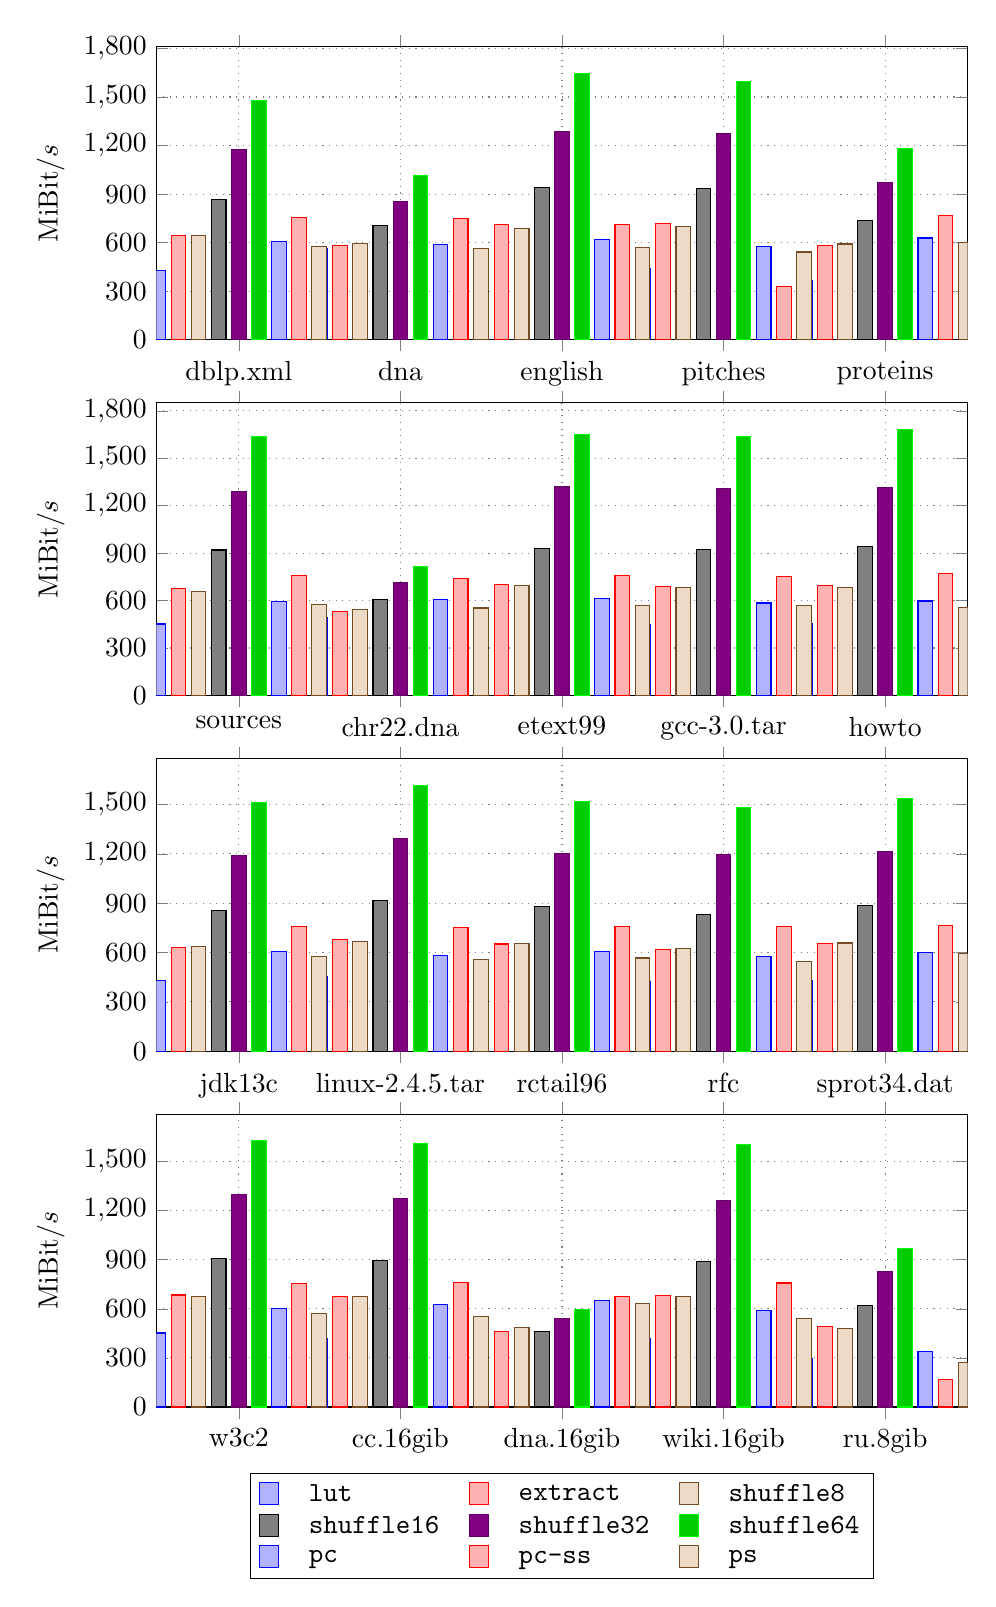
\begin{tikzpicture}
            \begin{groupplot} [
                width = 0.98\textwidth,
                height = 5.3cm,
                ybar,
                enlarge x limits = 0.1275,
                group style = { 
                    vertical sep = 0.8cm,
                    group size = { 
                        1 by 4
                    } 
                },
                ylabel = $\text{MiBit}/s$,
                legend style = { 
                    at = {(0.5, -0.225)},
                    anchor = north,
                    legend columns = 3,
                    column sep = 2ex
                },
                ytick distance = 300,
                symbolic x coords = {
                    dblp.xml,
                    dna,
                    english,
                    pitches,
                    proteins,
                    sources,
                    chr22.dna,
                    etext99,
                    gcc-3.0.tar,
                    howto,
                    jdk13c,
                    linux-2.4.5.tar,
                    rctail96,
                    rfc,
                    sprot34.dat,
                    w3c2,
                    cc.16gib,
                    dna.16gib,
                    wiki.16gib,
                    ru.8gib
                }
            ]
            
            
            \nextgroupplot [
                bar width = 0.185cm
            ]
    
    
                %% MULTIPLOT(type) SELECT file AS x, MEDIAN((height * (size / CAST(time_in_s AS Float))) / (1024 * 1024)) AS y,MULTIPLOT
                %% FROM stats WHERE (type LIKE 'wm%' OR type LIKE '%matrix') AND (file LIKE 'dblp.xml' OR file LIKE 'dna' OR file LIKE 'english' OR file LIKE 'pitches' OR file LIKE 'proteins') GROUP BY MULTIPLOT,x ORDER BY ds_order,MULTIPLOT,x
                \addplot coordinates { (dblp.xml,426.991) (dna,563.284) (english,451.729) (pitches,441.517) (proteins,363.248) };
                \addlegendentry{type=wm-lut-16-4-4};
                \addplot coordinates { (dblp.xml,643.493) (dna,584.094) (english,710.011) (pitches,716.518) (proteins,583.272) };
                \addlegendentry{type=wm-pext-8-8};
                \addplot coordinates { (dblp.xml,644.637) (dna,596.882) (english,689.463) (pitches,699.678) (proteins,591.187) };
                \addlegendentry{type=wm-shuffle-8-8};
                \addplot coordinates { (dblp.xml,864.114) (dna,703.218) (english,941.959) (pitches,934.417) (proteins,738.877) };
                \addlegendentry{type=wm-shuffle-16-8};
                \addplot coordinates { (dblp.xml,1177.97) (dna,856.087) (english,1288.87) (pitches,1274.39) (proteins,974.382) };
                \addlegendentry{type=wm-shuffle-32-8};
                \addplot coordinates { (dblp.xml,1479.64) (dna,1014.67) (english,1645.44) (pitches,1594.31) (proteins,1181.96) };
                \addlegendentry{type=wm-shuffle-64-8};
                \addplot coordinates { (dblp.xml,605.244) (dna,587.402) (english,620.104) (pitches,577.125) (proteins,628.283) };
                \addlegendentry{type=pwm-pc-matrix};
                \addplot coordinates { (dblp.xml,757.449) (dna,750.118) (english,709.471) (pitches,328.953) (proteins,768.579) };
                \addlegendentry{type=pwm-pc-ss-matrix};
                \addplot coordinates { (dblp.xml,578.153) (dna,560.948) (english,570.494) (pitches,541.875) (proteins,601.355) };
                \addlegendentry{type=pwm-ps-matrix};
    
        \legend{};
    
       \nextgroupplot [
        bar width = 0.185cm
    ]
    
    
        %% MULTIPLOT(type) SELECT file AS x, MEDIAN((height * (size / CAST(time_in_s AS Float))) / (1024 * 1024)) AS y,MULTIPLOT
        %% FROM stats WHERE (type LIKE 'wm%' OR type LIKE '%matrix') AND (file LIKE 'sources' OR file LIKE 'chr22.dna' OR file LIKE 'etext99' OR file LIKE 'gcc-3.0.tar' OR file LIKE 'howto') GROUP BY MULTIPLOT,x ORDER BY ds_order,MULTIPLOT,x
        \addplot coordinates { (chr22.dna,493.208) (etext99,460.731) (gcc-3.0.tar,451.361) (howto,457.827) (sources,451.855) };
        \addlegendentry{type=wm-lut-16-4-4};
        \addplot coordinates { (chr22.dna,530.713) (etext99,704.631) (gcc-3.0.tar,691.156) (howto,696.118) (sources,674.681) };
        \addlegendentry{type=wm-pext-8-8};
        \addplot coordinates { (chr22.dna,545.67) (etext99,694.343) (gcc-3.0.tar,680.398) (howto,681.546) (sources,659.914) };
        \addlegendentry{type=wm-shuffle-8-8};
        \addplot coordinates { (chr22.dna,605.324) (etext99,931.554) (gcc-3.0.tar,925.036) (howto,941.629) (sources,919.884) };
        \addlegendentry{type=wm-shuffle-16-8};
        \addplot coordinates { (chr22.dna,711.554) (etext99,1318.68) (gcc-3.0.tar,1311.08) (howto,1316.85) (sources,1290.54) };
        \addlegendentry{type=wm-shuffle-32-8};
        \addplot coordinates { (chr22.dna,818.438) (etext99,1649.86) (gcc-3.0.tar,1635.53) (howto,1683.62) (sources,1639.41) };
        \addlegendentry{type=wm-shuffle-64-8};
        \addplot coordinates { (chr22.dna,607.664) (etext99,613.619) (gcc-3.0.tar,584.678) (howto,597.162) (sources,591.97) };
        \addlegendentry{type=pwm-pc-matrix};
        \addplot coordinates { (chr22.dna,738.184) (etext99,757.495) (gcc-3.0.tar,754.438) (howto,772.629) (sources,758.435) };
        \addlegendentry{type=pwm-pc-ss-matrix};
        \addplot coordinates { (chr22.dna,552.974) (etext99,566.973) (gcc-3.0.tar,567.358) (howto,558.194) (sources,575.104) };
        \addlegendentry{type=pwm-ps-matrix};

    
        \legend{};
    
        \nextgroupplot [
            bar width = 0.185cm
        ]
    
        
        
            %% MULTIPLOT(type) SELECT file AS x, MEDIAN((height * (size / CAST(time_in_s AS Float))) / (1024 * 1024)) AS y,MULTIPLOT
            %% FROM stats WHERE (type LIKE 'wm%' OR type LIKE '%matrix') AND (file LIKE 'jdk13c' OR file LIKE 'sprot34.dat' OR file LIKE 'linux-2.4.5.tar' OR file LIKE 'rctail96' OR file LIKE 'rfc') GROUP BY MULTIPLOT,x ORDER BY ds_order,MULTIPLOT,x
            \addplot coordinates { (jdk13c,427.338) (linux-2.4.5.tar,451.534) (rctail96,430.666) (rfc,423.053) (sprot34.dat,429.022) };
            \addlegendentry{type=wm-lut-16-4-4};
            \addplot coordinates { (jdk13c,632.906) (linux-2.4.5.tar,681.025) (rctail96,652.249) (rfc,618.805) (sprot34.dat,655.159) };
            \addlegendentry{type=wm-pext-8-8};
            \addplot coordinates { (jdk13c,636.659) (linux-2.4.5.tar,669.555) (rctail96,654.373) (rfc,623.961) (sprot34.dat,658.105) };
            \addlegendentry{type=wm-shuffle-8-8};
            \addplot coordinates { (jdk13c,857.869) (linux-2.4.5.tar,915.917) (rctail96,878.1) (rfc,831.526) (sprot34.dat,887.443) };
            \addlegendentry{type=wm-shuffle-16-8};
            \addplot coordinates { (jdk13c,1188.03) (linux-2.4.5.tar,1292.73) (rctail96,1204.59) (rfc,1193.39) (sprot34.dat,1215.04) };
            \addlegendentry{type=wm-shuffle-32-8};
            \addplot coordinates { (jdk13c,1513.05) (linux-2.4.5.tar,1618.24) (rctail96,1520.02) (rfc,1482.27) (sprot34.dat,1535.61) };
            \addlegendentry{type=wm-shuffle-64-8};
            \addplot coordinates { (jdk13c,605.48) (linux-2.4.5.tar,583.491) (rctail96,603.808) (rfc,576.417) (sprot34.dat,599.77) };
            \addlegendentry{type=pwm-pc-matrix};
            \addplot coordinates { (jdk13c,758.037) (linux-2.4.5.tar,754.481) (rctail96,760.041) (rfc,756.406) (sprot34.dat,764.322) };
            \addlegendentry{type=pwm-pc-ss-matrix};
            \addplot coordinates { (jdk13c,575.071) (linux-2.4.5.tar,559.274) (rctail96,566.577) (rfc,544.731) (sprot34.dat,593.712) };
            \addlegendentry{type=pwm-ps-matrix};

    
            \legend{};
    
    
            \nextgroupplot [
                bar width = 0.185cm
            ]
        
            
            
                %% MULTIPLOT(type) SELECT file AS x, MEDIAN((height * (size / CAST(time_in_s AS Float))) / (1024 * 1024)) AS y,MULTIPLOT
                %% FROM stats WHERE (type LIKE 'wm%' OR type LIKE '%matrix') AND (file LIKE 'w3c2' OR file LIKE 'cc.16gib' OR file LIKE 'dna.16gib' OR file LIKE 'wiki.16gib' OR file LIKE 'ru.8gib') GROUP BY MULTIPLOT,x ORDER BY ds_order,MULTIPLOT,x
                \addplot coordinates { (cc.16gib,419.24) (dna.16gib,464.852) (ru.8gib,298.809) (w3c2,452.316) (wiki.16gib,417.959) };
                \addlegendentry{type=wm-lut-16-4-4};
                \addplot coordinates { (cc.16gib,677.655) (dna.16gib,461.728) (ru.8gib,489.259) (w3c2,684.491) (wiki.16gib,681.495) };
                \addlegendentry{type=wm-pext-8-8};
                \addplot coordinates { (cc.16gib,674.131) (dna.16gib,486.135) (ru.8gib,478.388) (w3c2,675.252) (wiki.16gib,676.951) };
                \addlegendentry{type=wm-shuffle-8-8};
                \addplot coordinates { (cc.16gib,897.612) (dna.16gib,463.934) (ru.8gib,621.947) (w3c2,905.555) (wiki.16gib,887.348) };
                \addlegendentry{type=wm-shuffle-16-8};
                \addplot coordinates { (cc.16gib,1273.88) (dna.16gib,538.621) (ru.8gib,825.982) (w3c2,1296.13) (wiki.16gib,1261.63) };
                \addlegendentry{type=wm-shuffle-32-8};
                \addplot coordinates { (cc.16gib,1610.08) (dna.16gib,594.277) (ru.8gib,968.329) (w3c2,1625.86) (wiki.16gib,1600.97) };
                \addlegendentry{type=wm-shuffle-64-8};
                \addplot coordinates { (cc.16gib,625.573) (dna.16gib,651.686) (ru.8gib,336.96) (w3c2,599.761) (wiki.16gib,588.448) };
                \addlegendentry{type=pwm-pc-matrix};
                \addplot coordinates { (cc.16gib,757.9) (dna.16gib,674.329) (ru.8gib,169.981) (w3c2,753.543) (wiki.16gib,757.642) };
                \addlegendentry{type=pwm-pc-ss-matrix};
                \addplot coordinates { (cc.16gib,550.256) (dna.16gib,633.351) (ru.8gib,270.279) (w3c2,573.217) (wiki.16gib,542.189) };
                \addlegendentry{type=pwm-ps-matrix};


    
    
                \legend {
                    \texttt{lut},
                    \texttt{extract},
                    \texttt{shuffle8},
                    \texttt{shuffle16},
                    \texttt{shuffle32},
                    \texttt{shuffle64},
                    \texttt{pc},
                    \texttt{pc-ss},
                    \texttt{ps}
                }
                
    
    
            \end{groupplot}
        \end{tikzpicture}
    \end{center}
    \caption{Construction time results for uncompressed matrixs. With the exception of cc.16gib, 512 bit construction always wins out.}
    \end{figure}

% NOW KANETA

% SQL DROP TABLE stats

% IMPORT-DATA stats ../results-pcc-regular.out
% IMPORT-DATA stats_kaneta ../results-kaneta-extrapolated.out

% SQL INSERT INTO stats SELECT * FROM stats_kaneta
% SQL INSERT INTO stats SELECT * FROM stats_lw

% SQL DELETE FROM stats WHERE type LIKE 'pwm%'
% SQL DELETE FROM stats WHERE type LIKE '%_lut_%'

% SQL UPDATE stats SET type = 'lwt-pext-16-4' WHERE type LIKE 'lwt_pext_16_4'
% SQL UPDATE stats SET type = 'lwt-shuffle-8-8' WHERE type LIKE 'lwt_shuffle_8_8'
% SQL UPDATE stats SET type = 'wm-pext-16-4' WHERE type LIKE 'wm_pext_16_4'
% SQL UPDATE stats SET type = 'wm-shuffle-8-8' WHERE type LIKE 'wm_shuffle_8_8'
% SQL UPDATE stats SET type = 'wt-kaneta-pext' WHERE type LIKE 'wt_kaneta_pext%'
% SQL UPDATE stats SET type = 'wt-kaneta-pshufb' WHERE type LIKE 'wt_kaneta_pshufb%'
% SQL UPDATE stats SET type = 'wm-kaneta-pext' WHERE type LIKE 'wm_kaneta_pext%'
% SQL UPDATE stats SET type = 'wm-kaneta-pshufb' WHERE type LIKE 'wm_kaneta_pshufb%'
% SQL DELETE FROM stats WHERE type LIKE '%\_%' ESCAPE '\'

% SQL UPDATE stats SET ds_order = 0 WHERE type LIKE '%pext-_%'
% SQL UPDATE stats SET ds_order = 1 WHERE type LIKE '%kaneta-pext'
% SQL UPDATE stats SET ds_order = 2 WHERE type LIKE '%shuffle-_%'
% SQL UPDATE stats SET ds_order = 3 WHERE type LIKE '%kaneta-pshufb'


% SQL UPDATE stats SET file = 'dblp.xml' WHERE file LIKE '%/dblp.xml'
% SQL UPDATE stats SET file = 'dna' WHERE file LIKE '%/dna'
% SQL UPDATE stats SET file = 'english' WHERE file LIKE '%/english'
% SQL UPDATE stats SET file = 'pitches' WHERE file LIKE '%/pitches'
% SQL UPDATE stats SET file = 'proteins' WHERE file LIKE '%/proteins'
% SQL UPDATE stats SET file = 'sources' WHERE file LIKE '%/sources'

% SQL UPDATE stats SET file = 'chr22.dna' WHERE file LIKE '%/chr22.dna'
% SQL UPDATE stats SET file = 'etext99' WHERE file LIKE '%/etext99'
% SQL UPDATE stats SET file = 'gcc-3.0.tar' WHERE file LIKE '%/gcc-3.0.tar'
% SQL UPDATE stats SET file = 'howto' WHERE file LIKE '%/howto'
% SQL UPDATE stats SET file = 'jdk13c' WHERE file LIKE '%/jdk13c'
% SQL UPDATE stats SET file = 'linux-2.4.5.tar' WHERE file LIKE '%/linux-2.4.5.tar'
% SQL UPDATE stats SET file = 'rctail96' WHERE file LIKE '%/rctail96'
% SQL UPDATE stats SET file = 'rfc' WHERE file LIKE '%/rfc'
% SQL UPDATE stats SET file = 'sprot34.dat' WHERE file LIKE '%/sprot34.dat'
% SQL UPDATE stats SET file = 'w3c2' WHERE file LIKE '%/w3c2'

\pgfplotsset{
  /pgfplots/bar cycle list/.style = {
    /pgfplots/cycle list = {
      { fill = green!65, mark = none },        % PEXT
      { fill = red!50, mark = none },          % KANETA PEXT
      { fill = blue!55, mark = none },         % PSHUFB 8-8
      { fill = orange!50, mark = none }        % KANETA PSHUFB
    }
  }
}


\begin{figure}
    \begin{center}
        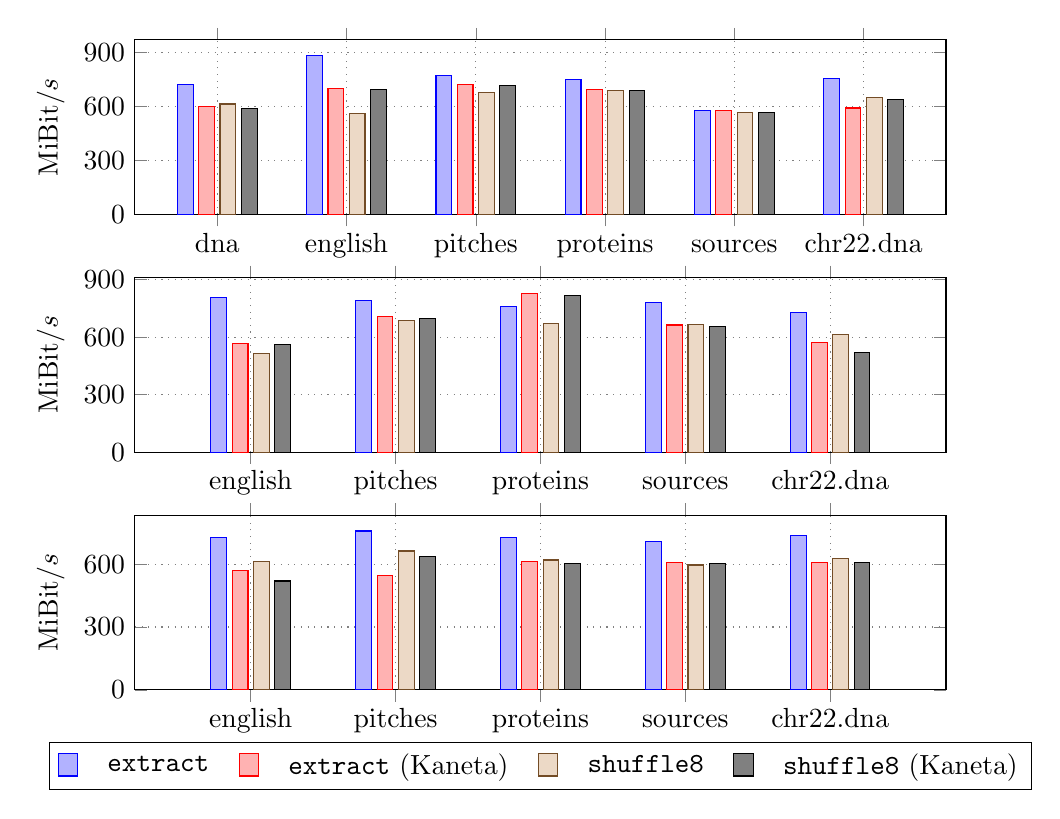
\begin{tikzpicture}
            \begin{groupplot} [
                width = 0.98\textwidth,
                height = 3.8cm,
                ybar,
                enlarge x limits = 0.1275,
                group style = { 
                    vertical sep = 0.8cm,
                    group size = { 
                        1 by 3
                    } 
                },
                ylabel = $\text{MiBit}/s$,
                legend style = { 
                    at = {(0.5, -0.3)},
                    anchor = north,
                    legend columns = -1,
                    column sep = 2ex
                },
                ytick distance = 300,
                symbolic x coords = {
                    dblp.xml,
                    dna,
                    english,
                    pitches,
                    proteins,
                    sources,
                    chr22.dna,
                    etext99,
                    gcc-3.0.tar,
                    howto,
                    jdk13c,
                    linux-2.4.5.tar,
                    rctail96,
                    rfc,
                    sprot34.dat,
                    w3c2
                },
                xticklabel style = {
                    text height = 1.35ex
                },
                xticklabels = {
                    dblp.xml\strut,
                    dna\strut,
                    english\strut,
                    pitches\strut,
                    proteins\strut,
                    sources\strut,
                    chr22.dna\strut,
                    etext99\strut,
                    gcc-3.0.tar\strut,
                    howto\strut,
                    jdk13c\strut,
                    linux-2.4.5.tar\strut,
                    rctail96\strut,
                    rfc\strut,
                    sprot34.dat\strut,
                    w3c2\strut
                }
            ]
            
            
            \nextgroupplot [
                bar width = 0.2cm
            ]
    
    
                %% MULTIPLOT(type) SELECT file AS x, MEDIAN((height * (size / CAST(time_in_s AS Float))) / (1024 * 1024)) AS y,MULTIPLOT
                %% FROM stats WHERE (type LIKE 'wt%' OR type LIKE 'lwt%') AND (file LIKE 'dblp.xml' OR file LIKE 'dna' OR file LIKE 'english' OR file LIKE 'pitches' OR file LIKE 'proteins' OR file LIKE 'sources') GROUP BY MULTIPLOT,x ORDER BY ds_order,MULTIPLOT,x
                \addplot coordinates { (dblp.xml,722.205) (dna,883) (english,770.548) (pitches,749.238) (proteins,575.985) (sources,757.753) };
                \addlegendentry{type=lwt-pext-16-4};
                \addplot coordinates { (dblp.xml,598.427) (dna,701.227) (english,721.176) (pitches,695.46) (proteins,575.917) (sources,591.891) };
                \addlegendentry{type=wt-kaneta-pext};
                \addplot coordinates { (dblp.xml,614.24) (dna,563.111) (english,677.957) (pitches,686.877) (proteins,565.628) (sources,650.216) };
                \addlegendentry{type=lwt-shuffle-8-8};
                \addplot coordinates { (dblp.xml,588.742) (dna,694.451) (english,715.091) (pitches,688.216) (proteins,566.598) (sources,636.845) };
                \addlegendentry{type=wt-kaneta-pshufb};
    
        \legend{};
    
       \nextgroupplot [
        bar width = 0.2cm,
        enlarge x limits = 0.2
    ]
    
    
        %% MULTIPLOT(type) SELECT file AS x, MEDIAN((height * (size / CAST(time_in_s AS Float))) / (1024 * 1024)) AS y,MULTIPLOT
        %% FROM stats WHERE (type LIKE 'wt%' OR type LIKE 'lwt%') AND (file LIKE 'chr22.dna' OR file LIKE 'etext99' OR file LIKE 'gcc-3.0.tar' OR file LIKE 'howto' OR file LIKE 'jdk13c') GROUP BY MULTIPLOT,x ORDER BY ds_order,MULTIPLOT,x
        \addplot coordinates { (chr22.dna,808.538) (etext99,790.826) (gcc-3.0.tar,760.615) (howto,779.279) (jdk13c,726.537) };
        \addlegendentry{type=lwt-pext-16-4};
        \addplot coordinates { (chr22.dna,566.048) (etext99,708.829) (gcc-3.0.tar,828.587) (howto,663.152) (jdk13c,570.669) };
        \addlegendentry{type=wt-kaneta-pext};
        \addplot coordinates { (chr22.dna,514.561) (etext99,687.514) (gcc-3.0.tar,673.4) (howto,667.552) (jdk13c,613.813) };
        \addlegendentry{type=lwt-shuffle-8-8};
        \addplot coordinates { (chr22.dna,562.441) (etext99,696.607) (gcc-3.0.tar,816.363) (howto,654.068) (jdk13c,519.728) };
        \addlegendentry{type=wt-kaneta-pshufb};
    
        \legend{};
    
        \nextgroupplot [
            bar width = 0.2cm,
            enlarge x limits = 0.2
        ]
    
        
        
            %% MULTIPLOT(type) SELECT file AS x, MEDIAN((height * (size / CAST(time_in_s AS Float))) / (1024 * 1024)) AS y,MULTIPLOT
            %% FROM stats WHERE (type LIKE 'wt%' OR type LIKE 'lwt%') AND (file LIKE 'jdk13c' OR file LIKE 'sprot34.dat' OR file LIKE 'linux-2.4.5.tar' OR file LIKE 'rctail96' OR file LIKE 'rfc') GROUP BY MULTIPLOT,x ORDER BY ds_order,MULTIPLOT,x
            \addplot coordinates { (jdk13c,726.537) (linux-2.4.5.tar,758.871) (rctail96,728.71) (rfc,709.137) (sprot34.dat,736.44) };
            \addlegendentry{type=lwt-pext-16-4};
            \addplot coordinates { (jdk13c,570.669) (linux-2.4.5.tar,547.424) (rctail96,612.237) (rfc,607.306) (sprot34.dat,607.861) };
            \addlegendentry{type=wt-kaneta-pext};
            \addplot coordinates { (jdk13c,613.813) (linux-2.4.5.tar,663.42) (rctail96,620.496) (rfc,596.415) (sprot34.dat,626.154) };
            \addlegendentry{type=lwt-shuffle-8-8};
            \addplot coordinates { (jdk13c,519.728) (linux-2.4.5.tar,635.854) (rctail96,601.947) (rfc,602.243) (sprot34.dat,607.861) };
            \addlegendentry{type=wt-kaneta-pshufb};

    
                \legend {
                    \texttt{extract},
                    \texttt{extract} (Kaneta),
                    \texttt{shuffle8},
                    \texttt{shuffle8} (Kaneta)
                }
                
    
    
            \end{groupplot}
        \end{tikzpicture}
    \end{center}
    \caption{Construction time results for uncompressed matrixs. With the exception of cc.16gib, 512 bit construction always wins out.}
    \end{figure}


\begin{figure}
    \begin{center}
        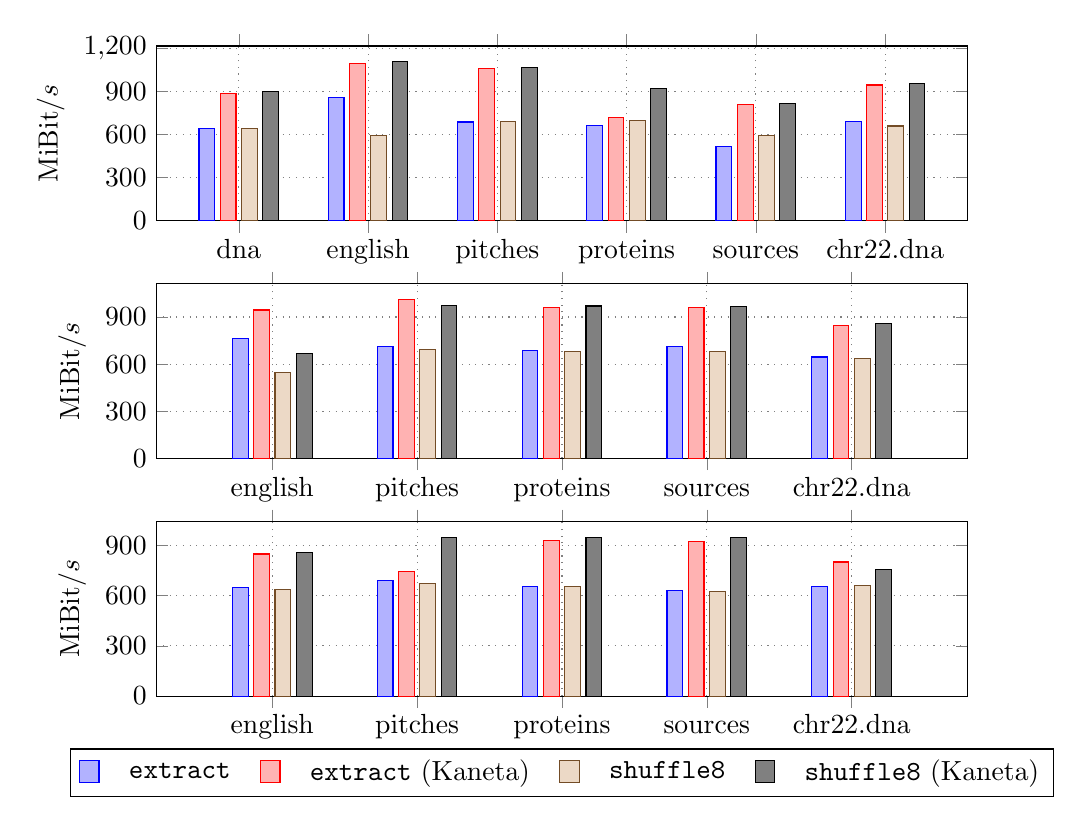
\begin{tikzpicture}
            \begin{groupplot} [
                width = 0.98\textwidth,
                height = 3.8cm,
                ybar,
                enlarge x limits = 0.1275,
                group style = { 
                    vertical sep = 0.8cm,
                    group size = { 
                        1 by 3
                    } 
                },
                ylabel = $\text{MiBit}/s$,
                legend style = { 
                    at = {(0.5, -0.3)},
                    anchor = north,
                    legend columns = -1,
                    column sep = 2ex
                },
                ytick distance = 300,
                symbolic x coords = {
                    dblp.xml,
                    dna,
                    english,
                    pitches,
                    proteins,
                    sources,
                    chr22.dna,
                    etext99,
                    gcc-3.0.tar,
                    howto,
                    jdk13c,
                    linux-2.4.5.tar,
                    rctail96,
                    rfc,
                    sprot34.dat,
                    w3c2
                },
                xticklabel style = {
                    text height = 1.35ex
                },
                xticklabels = {
                    dblp.xml\strut,
                    dna\strut,
                    english\strut,
                    pitches\strut,
                    proteins\strut,
                    sources\strut,
                    chr22.dna\strut,
                    etext99\strut,
                    gcc-3.0.tar\strut,
                    howto\strut,
                    jdk13c\strut,
                    linux-2.4.5.tar\strut,
                    rctail96\strut,
                    rfc\strut,
                    sprot34.dat\strut,
                    w3c2\strut
                }
            ]
            
            
            \nextgroupplot [
                bar width = 0.2cm
            ]
    
    
                %% MULTIPLOT(type) SELECT file AS x, MEDIAN((height * (size / CAST(time_in_s AS Float))) / (1024 * 1024)) AS y,MULTIPLOT
                %% FROM stats WHERE (type LIKE 'wm%') AND (file LIKE 'dblp.xml' OR file LIKE 'dna' OR file LIKE 'english' OR file LIKE 'pitches' OR file LIKE 'proteins' OR file LIKE 'sources') GROUP BY MULTIPLOT,x ORDER BY ds_order,MULTIPLOT,x
                \addplot coordinates { (dblp.xml,640.348) (dna,855.849) (english,687.986) (pitches,664.15) (proteins,515.541) (sources,690.288) };
                \addlegendentry{type=wm-pext-16-4};
                \addplot coordinates { (dblp.xml,885.721) (dna,1097.99) (english,1060.81) (pitches,721.67) (proteins,810.027) (sources,945.665) };
                \addlegendentry{type=wm-kaneta-pext};
                \addplot coordinates { (dblp.xml,644.637) (dna,596.882) (english,689.463) (pitches,699.678) (proteins,591.187) (sources,659.914) };
                \addlegendentry{type=wm-shuffle-8-8};
                \addplot coordinates { (dblp.xml,898.878) (dna,1106.5) (english,1067.52) (pitches,920.173) (proteins,818.942) (sources,957.707) };
                \addlegendentry{type=wm-kaneta-pshufb};
    
        \legend{};
    
       \nextgroupplot [
        bar width = 0.2cm,
        enlarge x limits = 0.2
    ]
    
    
        %% MULTIPLOT(type) SELECT file AS x, MEDIAN((height * (size / CAST(time_in_s AS Float))) / (1024 * 1024)) AS y,MULTIPLOT
        %% FROM stats WHERE (type LIKE 'wm%') AND (file LIKE 'chr22.dna' OR file LIKE 'etext99' OR file LIKE 'gcc-3.0.tar' OR file LIKE 'howto' OR file LIKE 'jdk13c') GROUP BY MULTIPLOT,x ORDER BY ds_order,MULTIPLOT,x
        \addplot coordinates { (chr22.dna,765.317) (etext99,711.151) (gcc-3.0.tar,689.007) (howto,709.471) (jdk13c,645.591) };
        \addlegendentry{type=wm-pext-16-4};
        \addplot coordinates { (chr22.dna,944.52) (etext99,1010.76) (gcc-3.0.tar,960.739) (howto,957.865) (jdk13c,847.194) };
        \addlegendentry{type=wm-kaneta-pext};
        \addplot coordinates { (chr22.dna,545.67) (etext99,694.343) (gcc-3.0.tar,680.398) (howto,681.546) (jdk13c,636.659) };
        \addlegendentry{type=wm-shuffle-8-8};
        \addplot coordinates { (chr22.dna,668.432) (etext99,970.48) (gcc-3.0.tar,969.845) (howto,967.606) (jdk13c,857.36) };
        \addlegendentry{type=wm-kaneta-pshufb};
    
        \legend{};
    
        \nextgroupplot [
            bar width = 0.2cm,
            enlarge x limits = 0.2
        ]
    
        
        
            %% MULTIPLOT(type) SELECT file AS x, MEDIAN((height * (size / CAST(time_in_s AS Float))) / (1024 * 1024)) AS y,MULTIPLOT
            %% FROM stats WHERE (type LIKE 'wm%') AND (file LIKE 'jdk13c' OR file LIKE 'sprot34.dat' OR file LIKE 'linux-2.4.5.tar' OR file LIKE 'rctail96' OR file LIKE 'rfc') GROUP BY MULTIPLOT,x ORDER BY ds_order,MULTIPLOT,x
            \addplot coordinates { (jdk13c,645.591) (linux-2.4.5.tar,688.067) (rctail96,654.199) (rfc,627.346) (sprot34.dat,653.504) };
            \addlegendentry{type=wm-pext-16-4};
            \addplot coordinates { (jdk13c,847.194) (linux-2.4.5.tar,741.191) (rctail96,930.108) (rfc,923.972) (sprot34.dat,799.693) };
            \addlegendentry{type=wm-kaneta-pext};
            \addplot coordinates { (jdk13c,636.659) (linux-2.4.5.tar,669.555) (rctail96,654.373) (rfc,623.961) (sprot34.dat,658.105) };
            \addlegendentry{type=wm-shuffle-8-8};
            \addplot coordinates { (jdk13c,857.36) (linux-2.4.5.tar,943.489) (rctail96,945.63) (rfc,947.335) (sprot34.dat,755.512) };
            \addlegendentry{type=wm-kaneta-pshufb};

    
                \legend {
                    \texttt{extract},
                    \texttt{extract} (Kaneta),
                    \texttt{shuffle8},
                    \texttt{shuffle8} (Kaneta)
                }
                
    
    
            \end{groupplot}
        \end{tikzpicture}
    \end{center}
    \caption{Construction time results for uncompressed matrixs. With the exception of cc.16gib, 512 bit construction always wins out.}
    \end{figure}

\end{document}


